\documentclass[
	%parspace, % Add vertical space between paragraphs
	%noindent, % No indentation of first lines in each paragraph
	%nohyp, % No hyphenation of words
	%twoside, % Double sided format
	%draft, % Quicker draft compilation without rendering images
	%final, % Set final to hide todos
]{elteikthesis}[2024/04/26]

% The minted package is also supported for source highlighting
% See elteikthesis_minted.tex for example
\usepackage[newfloat]{minted}
\usepackage[utf8]{inputenc}

\DeclareUnicodeCharacter{2124}{$\mathbb{Z}$}
\DeclareUnicodeCharacter{2095}{h}
\DeclareUnicodeCharacter{2261}{$\equiv$}

% Document's metadata
\title{Integers as a Higher Inductive Type} % title
\date{2024} % year of defense

% Author's metadata
\author{Zoltán Balázs}
\degree{Computer Science MSc}

% Superivsor(s)' metadata
\supervisor{Ambrus Kaposi Dr.} % internal supervisor's name
\affiliation{Associate Professor} % internal supervisor's affiliation
%\extsupervisor{Jane Doe} % external supervisor's name
%\extaffiliation{Senior Developer} % external supervisor's affiliation

% University's metadata
\university{Eötvös Loránd University} % university's name
\faculty{Faculty of Informatics} % faculty's name
\department{Dept. of Programming Language and Compilers} % department's name
\city{Budapest} % city
\logo{elte_cimer_szines} % logo

% Add bibliography file
\addbibresource{thesis.bib}

% The document
\begin{document}

% Set document language
%\documentlang{hungarian}
\documentlang{english}

% List of todos (not in the final document)
%\listoftodos[\todolabel]

% Title page (mandatory)
\maketitle
% Topic declaration page (mandatory) - can also be attached instead
%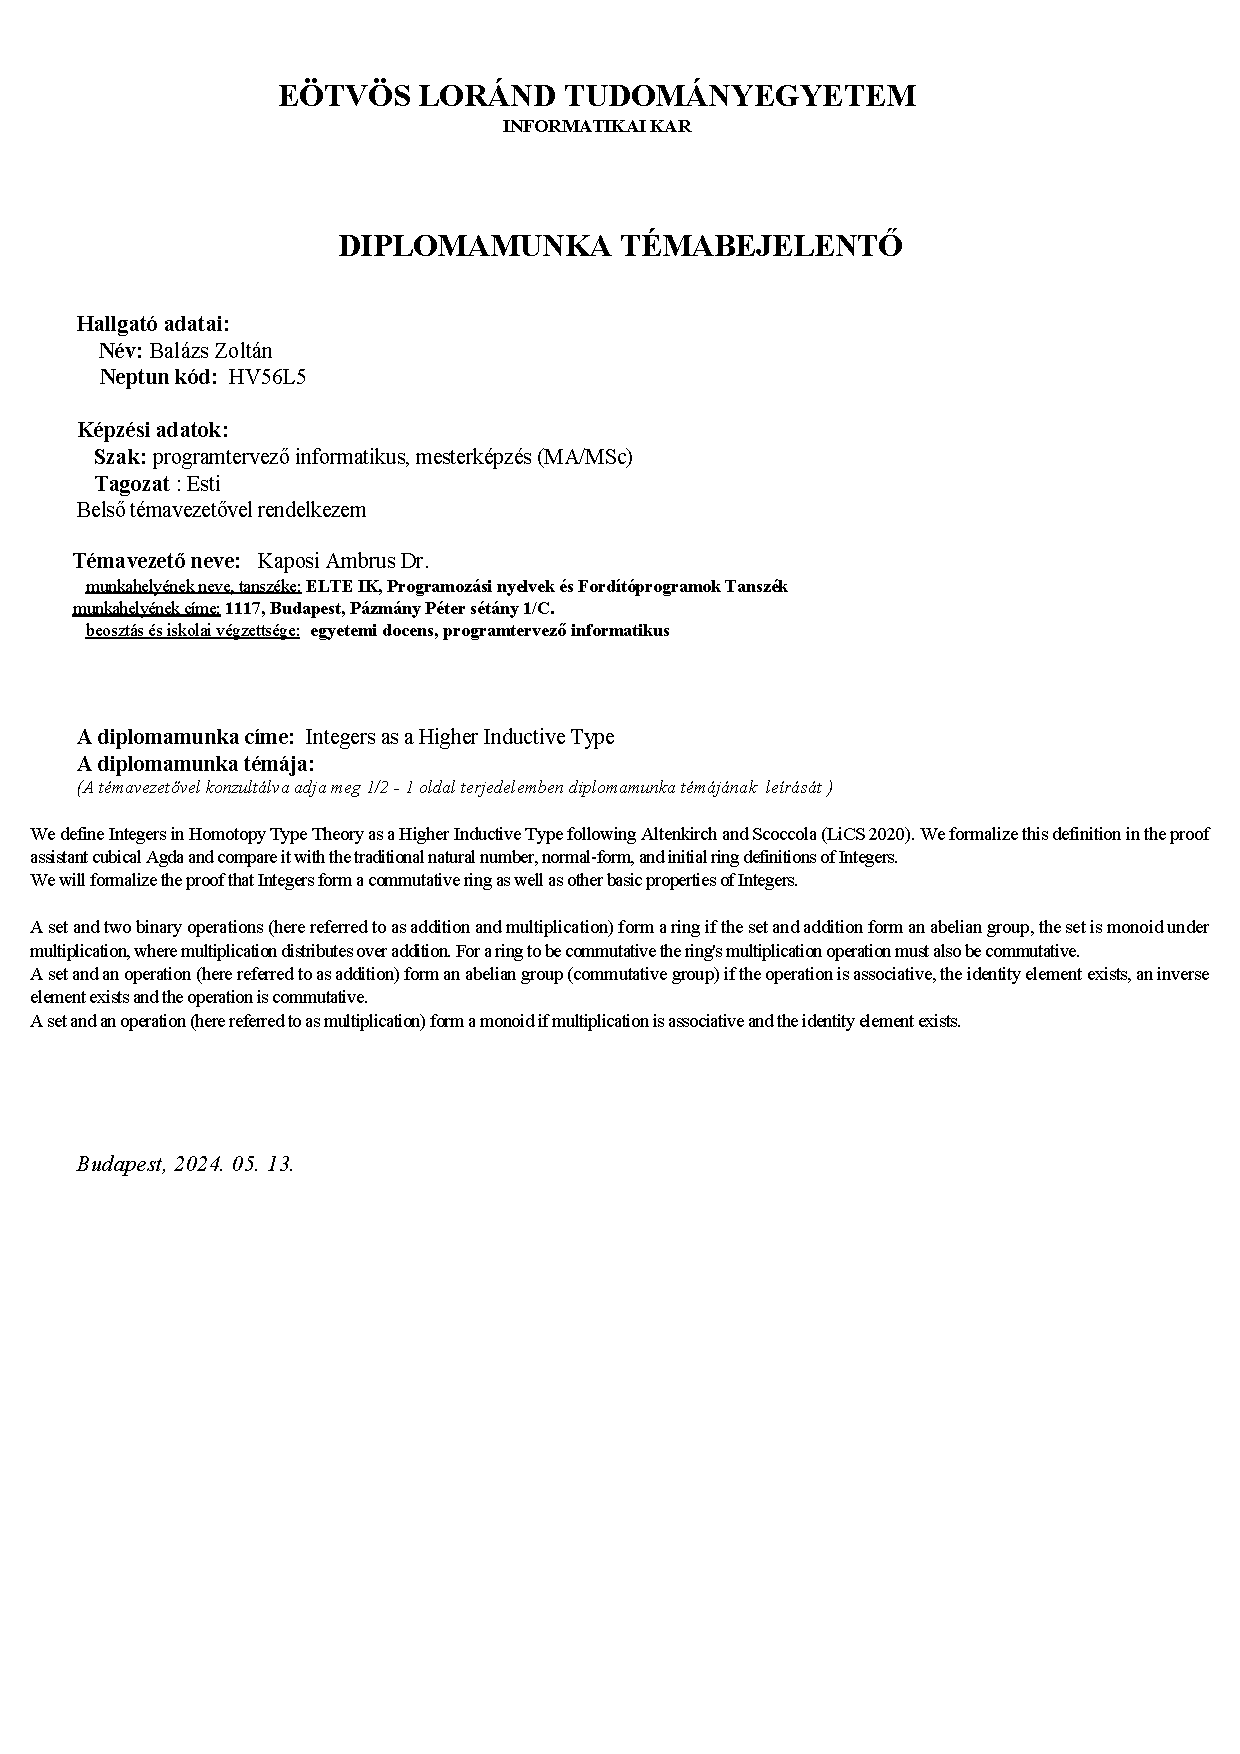
\includepdf{topicdeclaration.pdf}

% Table of contents (mandatory)
\tableofcontents
\cleardoublepage

% Main content
\chapter{Introduction}
\label{ch:intro}

\section{Type Definition}

In Homotopy Type Theory, we can define integers in numerous ways (one of them is using bi-invertible maps, which is a slightly less elegant version than ours\cite{10.1145/3373718.3394760}, since it involves 2 'pred' constructors, and ditches the 'coh' rule, in favour of being less complicated to prove properties. This bi-invertible map version is also included in the cubical Agda library\cite{biinv-agda}, which will prove useful for us), all with their own pros and cons. Following Paolo Capriotti's idea (presented by Thorsten Altenkirch\cite{bonn_2018}), our higher inductive type definition will be the following:
\begin{minted}{agda}
data ℤₕ : Set₀ where
  zero : ℤₕ
  succ : ℤₕ → ℤₕ
  pred : ℤₕ → ℤₕ
  sec : (z : ℤₕ) → pred (succ z) ≡ z
  ret : (z : ℤₕ) → succ (pred z) ≡ z
  coh : (z : ℤₕ) → congS succ (sec z) ≡ ret (succ z)
\end{minted}
With this definition, we have the base element 'zero', as well as 'succ' and 'pred' as constructors, to increment and decrement the integer value respectively. We then postulate that they are inverse to each other with the inclusion of 'sec' ('section', often seen in the Agda cubical library as 'predSuc') and 'ret' ('retraction', often seen as 'sucPred' in the same library). With a 'coh' ('coherence') constructor, we define an equivalence of equivalences, this constructor will introduce most of the challenges when trying to work with our integer definition. With the inclusion of this last condition, we also say that succ is a half-adjoint equivalence, something that we can use to our advantage in cubical Agda:
\begin{minted}{agda}
isHAℤₕ : isHAEquiv succ
isHAℤₕ .isHAEquiv.g    = pred
isHAℤₕ .isHAEquiv.linv = sec
isHAℤₕ .isHAEquiv.rinv = ret
isHAℤₕ .isHAEquiv.com  = coh
\end{minted}
Using this, we can define a sort of inverse coherence rule, a coherence that inverses the equivalence by applying 'pred' to 'ret', and checking that it is equal to passing the 'pred' value to 'sec':
\begin{minted}{agda}
hoc : (z : ℤₕ) → congS pred (ret z) ≡ sec (pred z)
hoc = com-op isHAℤₕ
\end{minted}
'com-op' simply uses the previously given fields and does the work for us, if our type is right, by correctly combining paths with 'hcomp' to match the wanted boundary.
This rule will be useful later on, when defining operations on our integer type. (Specifically when defining negation)

\section{Why Cubical Agda}

Since established that we want to use a Higher Inductive Type (HIT), which is not available in Martin-Löf Type Theory (MLTT). Agda, by default, doesn't support HITs as it is based on MLTT; an extension of it does however support CTT. While HoTT can essentially be summarized\cite{hottbook} by being MLTT with an additional Univalence axiom (where univalence states the following: (A ≃ B) ≃ (A = B), where A and B are types). Cubical Agda doesn't directly support HoTT; instead, it is a closely related version of Type Theory called Cubical Type Theory (CTT). CTT instead can be summarized as MLTT, with the interval type and its rules, the transport function and its rules, the glue type and hcomp. In CTT, univalence will not be an axiom but something that can be proven\cite{cohen2016cubicaltypetheoryconstructive}.

Since we need to use a proof assistant that supports HITs, which CTT supports,\cite{coquand2018higherinductivetypescubical}, we are forced to use Cubical Agda\cite{10.1145/3341691}, as there are no other proof assistants that do so. This will definitionally bring the added work that we will be forced to satisfy the boundaries required, as of the writing of this paper, there is no automatic way for these to be filled, but that might be subject to change\cite{doré2024automatingboundaryfillingcubical}.

The main benefit of our HIT integers will be that we can eliminate to higher dimensions (more specifically, above set, for example, to groupoid). The same could be said about Bi-Invertible integers, which use 2 'pred' constructors instead, and ditch the 'coherent' rule, however, a single 'pred' constructor with a 'coherent' rule is more elegant. There is also a definition of integers with the added 'isSet' constructor, while you could also eliminate with this version, you couldn't eliminate above set. Moreover, when defining your indunction property, you would also have to define the case for the 'isSet' constructor.

\section{Commutative Ring}
Our question is the following: Is this definition of integers a correct one, is it a set with decidable equality, and if so, do they form a commutative ring? (While this should be fairly obvious, integers do form a commutative ring, with the higher inductive type definition of integers, this hasn't been formally proven yet.) Moreover, what does it mean for integers to form a commutative ring? We will have to prove the following:

\begin{compactitem}
  \item The set and two binary operations (here: addition and multiplication) form a ring:
  \begin{compactitem}
    \item The set and addition form an abelian group:
    \begin{compactitem}
    \item Addition is associative
    \item The identity element exists
    \item An inverse element exists
    \item Addition is commutative
    \end{compactitem}
  \item The set is monoid under multiplication:
    \begin{compactitem}
    \item Multiplication is associative
    \item The identity element exists
    \end{compactitem}
  \item Multiplication distributes over addition
  \end{compactitem}
  \item Multiplication is commutative
\end{compactitem}
Before we prove these, we will dive into proving some other useful properties first.

\cleardoublepage

\chapter{Proving that HIT Integers Form a Set}
\label{ch:set}
This will be the first quite labours property to define. To make our live easier in the future, we will have to prove that our definition of integers actually form a set. To prove this, we will prove that our definition of integers is isomorphic with the standard definition of integers in cubical Agda:
\begin{minted}{agda}
data ℤ : Type₀ where
  pos    : (n : ℕ) → ℤ
  negsuc : (n : ℕ) → ℤ
\end{minted}
To do this, we will need to define 4 functions:
\begin{compactitem}
  \item We can convert our type to the standard integer definition
  \item We can convert from the standard integer definition to our type
  \item Converting the standard integer definition to our type, and back to the standard integer definition results in the exact same value
  \item Converting our type to the standard integer definition, and back to our type results in the exact same value
\end{compactitem}
This is a sort of pseudo comparison of the standard integer type and our type as well, if we prove that our type is isomorphic with the standard integer type, then the two types are equivalent as well.

Note: We could also go the way of defining that our HIT integers are discrete. One of the main points of the thesis is to compare different integer definitions to the HIT integers, so we will try to do less work and prove that our HIT integers form a set while comparing them to the standard integer definition. This also brings the quite fortunate side-effect that any other integer definitions that also prove isomorphism with the standard integers (in the cubical library one notable example is the previously mentioned bi-invertible integers) also, by extension, are isomorphic with our HIT integers.

Let us begin with proving the equivalence between standard integers and HIT integers.

\section{Converting our type to the standard definition}
First off, we will define the function to convert from our type to the standard integer type. We will do so by pattern matching on our integer value. This will give us all the cases for our constructors, for which we will need to provide an equivalent standard integer value. For our 'zero' value, the equivalent standard integer value is 'pos zero'. For our 'succ z' case, we will need to increment the value with 'sucℤ' and recursively convert the rest by calling our conversion function with 'z'. 'sucℤ' is defined for the standard integers, its purpose is to increment the standard integer value by one. For our 'pred z' case we will do the same thing, just with 'predℤ', as one might imagine, 'predℤ' is responsible for decrementing the standard integer value by one. The next case is the first truly interesting one, as we will have to convert a 'sec' integer to a standard integer value. As previously mentioned 'sec' is responsible for the equivalence of \mintinline{agda}{pred (succ z) ≡ z}. As such, we will not only need to give an appropriate standard integer value, but also satisfy the boundaries as stated by Agda:
\begin{minted}{agda}
i = i0 ⊢ predℤ (sucℤ (ℤₕ-ℤ z))
i = i1 ⊢ ℤₕ-ℤ z
\end{minted}
These boundaries match what our 'sec' constructor state, just for the standard integer values. (Note that instead of our integer type, we are dealing with the converted standard integer values, as such, we are basically proving that \mintinline{agda}{predℤ (sucℤ (ℤₕ-ℤ z)) ≡ ℤₕ-ℤ z}). Thankfully for us, there is a function in the standard library for this exact case called 'predSuc', this provides the exact boundary we need: \mintinline{agda}{∀ z → predℤ (sucℤ z) ≡ z}, as before, we will need to recursively call with the converted remaining integer value, as well as to pass the boundary 'i', as without that, it is just an equivalence, but giving the 'i' boundary resolves it to a standard integer value.
This is also the case for our 'ret' constructor, we will just need to use the standard 'sucPred' function, which is exactly what we need to satisfy the boundaries. (The wanted boundary is also different, to reflect the fact that we need to prove that 'ret' is defined as \mintinline{agda}{succ (pred z) ≡ z}.)
Our last constructor is 'coh', for which we will need a standard integer value and satisfy the needed boundaries. We will define the 'coh' rule for the standard integers. Following the cubical library, we will pattern match, do cover the 'pos n', 'negsuc zero' and 'negsuc (suc n)' cases. All of these cases result in a reflection, thanks to the way that 'sucℤ', 'predSuc' and 'sucPred' are defined.
\begin{minted}{agda}
cohℤ : ∀ z → congS sucℤ (predSuc z) ≡ sucPred (sucℤ z)
cohℤ (pos n)          = refl
cohℤ (negsuc zero)    = refl
cohℤ (negsuc (suc n)) = refl
\end{minted}

Note: the wanted boundaries for the conversion's 'coh' branch are as such:
\begin{minted}{agda}
j = i0 ⊢ sucℤ (predℤ (sucℤ (ℤₕ→ℤ z)))
j = i1 ⊢ sucℤ (ℤₕ→ℤ z)
i = i0 ⊢ sucℤ (predSuc (ℤₕ→ℤ z) j)
i = i1 ⊢ sucPred (sucℤ (ℤₕ→ℤ z)) j
\end{minted}
these exactly correspond to what the 4 parts of our 'coh' rule are, just with the standard integer functions and values. When using the 'coh' rule defined for the standard integers, we will have to convert our HIT integer to a standard integer, as well as providez both of our original boundaries.

Rewriting these wanted boundaries in Agda to a Square results in the following:
\[
\begin{tikzcd}
	\bullet &&&& \bullet \\
	\\
	\\
	\\
	\bullet &&&& \bullet
	\arrow["{suc\mathbb{Z}\:(\mathbb{Z}_h\shorttextrightarrow\mathbb{Z}\:z)}"{description}, no head, from=1-1, to=1-5]
	\arrow["{suc\mathbb{Z}\:(predSuc\:(\mathbb{Z}_h\shorttextrightarrow\mathbb{Z}\:z)\:j)}"{description}, no head, from=5-1, to=1-1]
	\arrow["{suc\mathbb{Z}\:(pred\mathbb{Z}\:(suc\mathbb{Z}\:(\mathbb{Z}_h\shorttextrightarrow\mathbb{Z}\:z)))}"{description}, no head, from=5-1, to=5-5]
	\arrow["{sucPred\:(suc\mathbb{Z}\:(\mathbb{Z}_h\shorttextrightarrow\mathbb{Z}\:z))\:j}"{description}, no head, from=5-5, to=1-5]
\end{tikzcd}
\]

\begin{listing}[H]
\begin{minted}{agda}
ℤₕ→ℤ : ℤₕ → ℤ
ℤₕ→ℤ zero        = pos zero
ℤₕ→ℤ (succ z)    = sucℤ (ℤₕ→ℤ z)
ℤₕ→ℤ (pred z)    = predℤ (ℤₕ→ℤ z)
ℤₕ→ℤ (sec z i)   = predSuc (ℤₕ→ℤ z) i
ℤₕ→ℤ (ret z i)   = sucPred (ℤₕ→ℤ z) i
ℤₕ→ℤ (coh z i j) = cohℤ (ℤₕ→ℤ z) i j
\end{minted}
\caption{Agda code for converting between HIT and the standard integers}
\end{listing}

\section{Converting the standard definition to our type}
Converting from the standard definition to our type turns out to be easier than the vice-versa. Pattern matching on both parameters (the default 'n' parameter, then the expanded 'pos n' and 'negsuc n' parameter) introduces four cases. We need to remember that 'pos zero' is equivalent to our 'zero' constructor, 'pos (suc n)' is equivalent to applying our 'succ' constructor, to the recursively converted 'pos n' value. 'negsuc' is an interesting case, as it is definitionally introduces '-1' to the value, so 'negsuc zero' is equivalent to '0 - 1', which is our 'pred zero', equivalently, 'negsuc (suc n)' is equivalent to applying 'pred' to the recursively converted 'negsuc n' value.
\begin{listing}[H]
\begin{minted}{agda}
ℤ→ℤₕ : ℤ → ℤₕ
ℤ→ℤₕ (pos zero)       = zero
ℤ→ℤₕ (pos (suc n))    = succ (ℤ→ℤₕ (pos n))
ℤ→ℤₕ (negsuc zero)    = pred zero
ℤ→ℤₕ (negsuc (suc n)) = pred (ℤ→ℤₕ (negsuc n))
\end{minted}
\caption{Agda code for converting between standard integers and HIT integers}
\end{listing}

\section{Converting the standard definition to our type and back}
Converting to and from isn't enough, we have to also ensure that if we are to convert a standard integer to our type, then that value in our type back to the standard integer, we get the same initial value.

As we did before, it is beneficial to pattern match to get the constructors of the standard integers. It turns out that if pattern match once again on the two constructors (so we get 'pos zero', 'pos (suc n)', 'negsuc zero' and 'negsuc (suc n)' cases), two of the four cases ('pos zero' and 'negsuc zero') become reflections. (Thanks to the way we defined 'ℤ→ℤₕ' and 'ℤₕ→ℤ' for the previously mentioned two cases, and 'zero' as well as 'pred zero')

Let's deal with the remaining two cases:

For 'pos (suc n)', we will have to prove the following: sucℤ (ℤₕ→ℤ (ℤ→ℤₕ (pos n))) ≡ pos (suc n). Note that more than likely we will need to recursively call the ℤ→ℤₕ→ℤ function with the remaining 'pos n' value, so let's do so. If we do this, suddenly we will already have the following: ℤₕ→ℤ (ℤ→ℤₕ (pos n)) ≡ pos n. Following the left-hand side, we will use congruence to apply the missing 'sucℤ' on both sides, this has the additional benefit that thanks to the definition of 'sucℤ', the right-hand side sucℤ (pos n) is definitionally equal to pos (suc n), the exact same thing we need.

For 'negsuc (suc n)' the story is quite similar. We need to prove the following: predℤ (ℤₕ→ℤ (ℤ→ℤₕ (negsuc n))) ≡ negsuc (suc n), we have the intuition of the recursive call with 'negsuc n' value, doing so results in ℤₕ→ℤ (ℤ→ℤₕ (negsuc n)) ≡ negsuc n, applying 'predℤ' to match the left-hand side brings the additional benefit that definitionally predℤ (negsuc n) is equal to negsuc (suc n), exactly what we need.

\begin{listing}[H]
\begin{minted}{agda}
ℤ→ℤₕ→ℤ : (z : ℤ) → ℤₕ→ℤ (ℤ→ℤₕ z) ≡ z
ℤ→ℤₕ→ℤ (pos zero)       = refl
ℤ→ℤₕ→ℤ (pos (suc n))    = cong sucℤ (ℤ→ℤₕ→ℤ (pos n))
ℤ→ℤₕ→ℤ (negsuc zero)    = refl
ℤ→ℤₕ→ℤ (negsuc (suc n)) = cong predℤ (ℤ→ℤₕ→ℤ (negsuc n))
\end{minted}
\caption{Agda proof that converting standard integers to HIT integers and back results in the same value}
\end{listing}
ℤ-ℤₕ-sucℤ : (z : ℤ) → ℤ-ℤₕ (sucℤ z) ≡ succ (ℤ-ℤₕ z)
ℤ-ℤₕ-sucℤ (pos n)          = refl
ℤ-ℤₕ-sucℤ (negsuc zero)    = sym (ret (ℤ-ℤₕ (pos zero)))
ℤ-ℤₕ-sucℤ (negsuc (suc n)) = sym (ret (ℤ-ℤₕ (negsuc n)))

ℤ-ℤₕ-predℤ : (z : ℤ) → ℤ-ℤₕ (predℤ z) ≡ pred (ℤ-ℤₕ z)
ℤ-ℤₕ-predℤ (pos zero)    = refl
ℤ-ℤₕ-predℤ (pos (suc n)) = sym (sec (ℤ-ℤₕ (pos n)))
ℤ-ℤₕ-predℤ (negsuc n)    = refl

sym-filler : ∀ {ℓ} {A : Type ℓ} {x y : A} (p : x ≡ y)
                → Square (sym p)
                         refl
                         refl
                         p
sym-filler p i j = p (i ∨ ~ j)

ℤ-ℤₕ-sucPred : (z : ℤ)
              → Square (ℤ-ℤₕ-sucℤ (predℤ z) ∙ (λ j → succ (ℤ-ℤₕ-predℤ z j)))
                       (λ _ → ℤ-ℤₕ z)
                       (λ i → ℤ-ℤₕ (sucPred z i))
                       (ret (ℤ-ℤₕ z))
ℤ-ℤₕ-sucPred (pos zero) i j =
  hcomp (λ k → λ { (j = i0) → ℤ-ℤₕ (pos zero)
                 ; (i = i0) → rUnit (sym (ret (ℤ-ℤₕ (pos zero)))) k j
                 ; (i = i1) → ℤ-ℤₕ (pos zero)
                 ; (j = i1) → ret (ℤ-ℤₕ (pos zero)) i
                 })
        (sym-filler (ret (ℤ-ℤₕ (pos zero))) i j)
ℤ-ℤₕ-sucPred (pos (suc n)) i j =
  hcomp (λ k → λ { (j = i0) → succ (ℤ-ℤₕ (pos n))
                 ; (i = i0) → lUnit (λ i → succ (sym (sec (ℤ-ℤₕ (pos n))) i)) k j
                 ; (i = i1) → succ (ℤ-ℤₕ (pos n))
                 ; (j = i1) → coh (ℤ-ℤₕ (pos n)) k i
                 })
        (succ (sym-filler (sec (ℤ-ℤₕ (pos n))) i j))
ℤ-ℤₕ-sucPred (negsuc n) i j =
  hcomp (λ k → λ { (j = i0) → ℤ-ℤₕ (negsuc n)
                 ; (i = i0) → rUnit (sym (ret (ℤ-ℤₕ (negsuc n)))) k j
                 ; (i = i1) → ℤ-ℤₕ (negsuc n)
                 ; (j = i1) → ret (ℤ-ℤₕ (negsuc n)) i
                 })
        (sym-filler (ret (ℤ-ℤₕ (negsuc n))) i j)

ℤ-ℤₕ-predSuc : (x : ℤ)
              → Square (ℤ-ℤₕ-predℤ (sucℤ x) ∙ (λ i → pred (ℤ-ℤₕ-sucℤ x i)))
                       (λ _ → ℤ-ℤₕ x)
                       (λ i → ℤ-ℤₕ (predSuc x i))
                       (sec (ℤ-ℤₕ x))
ℤ-ℤₕ-predSuc (pos n) i j =
    hcomp (λ k → λ { (j = i0) → ℤ-ℤₕ (pos n)
                   ; (i = i0) → rUnit (sym (sec (ℤ-ℤₕ (pos n)))) k j
                   ; (i = i1) → ℤ-ℤₕ (pos n)
                   ; (j = i1) → sec (ℤ-ℤₕ (pos n)) i
                   })
          (sym-filler (sec (ℤ-ℤₕ (pos n))) i j)
ℤ-ℤₕ-predSuc (negsuc zero) i j =
    hcomp (λ k → λ { (j = i0) → ℤ-ℤₕ (negsuc zero)
                   ; (i = i0) → lUnit (λ i → pred (sym (ret (ℤ-ℤₕ (pos zero))) i)) k j
                   ; (i = i1) → ℤ-ℤₕ (negsuc zero)
                   ; (j = i1) → hoc (ℤ-ℤₕ (pos zero)) k i
                   })
          (pred (sym-filler (ret (ℤ-ℤₕ (pos zero))) i j))
ℤ-ℤₕ-predSuc (negsuc (suc n)) i j =
    hcomp (λ k → λ { (j = i0) → ℤ-ℤₕ (negsuc (suc n))
                   ; (i = i0) → lUnit (λ i → pred (sym (ret (ℤ-ℤₕ (negsuc n))) i)) k j
                   ; (i = i1) → ℤ-ℤₕ (negsuc (suc n))
                   ; (j = i1) → hoc (ℤ-ℤₕ (negsuc n)) k i
                   })
          (pred (sym-filler (ret (ℤ-ℤₕ (negsuc n))) i j))

ℤₕ-ℤ-ℤₕ zero          = refl
ℤₕ-ℤ-ℤₕ (succ z)      = ℤ-ℤₕ-sucℤ (ℤₕ-ℤ z) ∙ (λ i → succ (ℤₕ-ℤ-ℤₕ z i))
ℤₕ-ℤ-ℤₕ (pred z)      = ℤ-ℤₕ-predℤ (ℤₕ-ℤ z) ∙ (λ i → pred (ℤₕ-ℤ-ℤₕ z i))
ℤₕ-ℤ-ℤₕ (sec z i) j   =
  hcomp (λ k → λ { (j = i0) → ℤ-ℤₕ (predSuc (ℤₕ-ℤ z) i)
                 ; (i = i0) → (ℤ-ℤₕ-predℤ (sucℤ (ℤₕ-ℤ z)) ∙ (λ i → pred (compPath-filler (ℤ-ℤₕ-sucℤ (ℤₕ-ℤ z))
                     (λ i' → succ (ℤₕ-ℤ-ℤₕ z i'))
                     k i))) j
                 ; (i = i1) → ℤₕ-ℤ-ℤₕ z (j ∧ k)
                 ; (j = i1) → sec (ℤₕ-ℤ-ℤₕ z k) i })
        (ℤ-ℤₕ-predSuc (ℤₕ-ℤ z) i j)
ℤₕ-ℤ-ℤₕ (ret z i) j   =
  hcomp (λ k → λ { (j = i0) → ℤ-ℤₕ (sucPred (ℤₕ-ℤ z) i)
                 ; (i = i0) → (ℤ-ℤₕ-sucℤ (predℤ (ℤₕ-ℤ z)) ∙ (λ i → succ (compPath-filler (ℤ-ℤₕ-predℤ (ℤₕ-ℤ z))
                     (congS pred (ℤₕ-ℤ-ℤₕ z))
                     k i))) j
                 ; (i = i1) → ℤₕ-ℤ-ℤₕ z (j ∧ k)
                 ; (j = i1) → ret (ℤₕ-ℤ-ℤₕ z k) i  })
        (ℤ-ℤₕ-sucPred (ℤₕ-ℤ z) i j)
ℤₕ-ℤ-ℤₕ (coh z i j) k = ?
\end{minted}

\subsection{Set property}
With these 4 functions defined, we can prove that our type is isomorphic with the standard definition:
\begin{minted}[fontsize=\small]{agda}
ℤ-iso : Iso ℤ ℤₕ
ℤ-iso .Iso.fun      = ℤ-ℤₕ
ℤ-iso .Iso.inv      = ℤₕ-ℤ
ℤ-iso .Iso.rightInv = ℤₕ-ℤ-ℤₕ
ℤ-iso .Iso.leftInv  = ℤ-ℤₕ-ℤ

ℤ≡ℤₕ : ℤ ≡ ℤₕ
ℤ≡ℤₕ = isoToPath ℤ-iso
\end{minted}
We pattern match on the constructors of $Iso$ (isomorphism) and we provide the needed fields. (As discussed earlier.)

Finally, we can use the fact that the standard definition forms a set to our advantage, as our type is isomorphic with the standard definition means that our type also forms a set:
\begin{minted}{agda}
isSetℤₕ : isSet ℤₕ
isSetℤₕ = subst isSet ℤ≡ℤₕ isSetℤ
\end{minted}

\cleardoublepage

\chapter{Abelian Group (Addition)}
\label{ch:abgroup}

\section{Addition Operation}
To define addition, we will use our iterator. For this, we will need an equivalence, in this simpler case we will first define an isomorphism, then convert that to an equivalence.
This isomorphism will be based on 'succ' being the function, its inverse function will be 'pred', and to prove that using 'succ' then 'pred', and using 'pred' then 'succ' results in the same value, we will use our 'section' and 'retraction' constructors.

We can then convert this isomorphism to an equivalence with the 'isoToEquiv' builtin function. Equivalence is an ordered pair, where the first parameter will be our 'succ' function, and the second will contain the proofs we previously mentioned.

Using the iterator we defined earlier, we can first supply the 'idfun' (identity function) version of ℤₕ, this will convert ℤₕ to a 'ℤₕ → ℤₕ' type. This will be beneficial since we have 2 implicit parameters, and we will want to move the constructors ('succ' and 'pred') from the left parameter to the right one. Next, we will post-compose our defined 'succEquiv'. This will change our 'ℤₕ ≃ ℤₕ' to a '(ℤₕ → ℤₕ) ≃ (ℤₕ → ℤₕ)' (more specifically (C → ℤₕ) ≃ (C → ℤₕ)), this is to match the type needed by our iterator. We implicitly supply the left and right parameters to this. (More specifically, we will first supply our left parameter, for this our iterator will return ℤₕ → ℤₕ, and we will supply our right parameter to this - see the comment in the code for this).

This will have the desired effect that we wanted: from our left parameter the 'succ' and 'pred' constructors will be placed on the beginning of the right parameter, which is otherwise known as addition.

As we already established when defining our iterator, we won't have to deal with our 1- and 2-dimensional construcotrs and their boundaries, as it is handled by our iterator.

\begin{minted}{agda}
succIso : Iso ℤₕ ℤₕ
succIso .Iso.fun      = succ
succIso .Iso.inv      = pred
succIso .Iso.rightInv = ret
succIso .Iso.leftInv  = sec

succEquiv : ℤₕ ≃ ℤₕ
succEquiv = isoToEquiv succIso

infixl 6 _+_
_+_ : ℤₕ → ℤₕ → ℤₕ
_+_ = ℤₕ-ite (idfun ℤₕ) (postCompEquiv succEquiv)
-- m + n = (ℤₕ-ite (idfun ℤₕ) (postCompEquiv succEquiv) m) n
\end{minted}

Definitionally, the following hold true for the addition operation in Agda:
\begin{minted}{agda}
zero   + n ≡ n
succ m + n ≡ succ (m + n)
pred m + n ≡ pred (m + n)
\end{minted}
Note that the symmetric version of these also hold true.

Alternatively, we could define addition by pattern matching on the second parameter, this would mean we manually have to satisfy the boundaries in the 1- and 2-dimensional constructor cases, however, here they would be fairly trivial:
% !!BOUNDARY!!
\begin{minted}{agda}
_+_ : ℤₕ → ℤₕ → ℤₕ
zero      + b = b
succ a    + b = succ (a + b)
pred a    + b = pred (a + b)
sec a i   + b = sec (a + b) i
ret a i   + b = ret (a + b) i
coh a i j + b = coh (a + b) i j
\end{minted}

\section{Associativity}
\begin{theorem}
  Addition is associative: ∀ m, n, o ∈ ℤ: m + (n + o) = (m + n) + o
\end{theorem}

\begin{proof}
  We will use our induction property to prove this theorem. For the first case, which states that this is indeed a property, we will use the 'isProp' (specifically the one which takes 2 parameters) and our set property, thankfully cubical Agda can infer the parameters for this. In all future proofs we will rely on Agda inferring these parameters.

  For the base case (m = 0) : 0 + (n + o) = (n + o) = (0 + n) + o is a reflection.

  For the succ case: (succ m) + (n + o) = ((succ m) + n) + o, note that since we are using the induction property, we will have the original m + (n + o) = (m + n) + o equality, where we are free to change the parameters of 'n' and 'o' as we please. Applying succ to the original equality will result in succ (m + (n + o)) = succ (m + n + o), thanks to the fact that succ (m + n) = succ m + n holds true definitionally, where we can supply 'm' to the m parameter, and 'n + o' to the n parameter. We will also have to note that addition is parenthesized from the left, so succ m + n + o = (succ m + n) + o is also definitionally true.

  For the pred case: (pred m) + (n + o) = ((pred m) + n) + o, similarly to the succ case, it is enough to apply pred to the original equality. We will once again note that pred (m + n) = pred m + n is definitionally true, and the fact that addition is parenthesized from the left.
\end{proof}

\begin{listing}[H]
\begin{minted}{agda}
+-assoc : ∀ m n o → m + (n + o) ≡ (m + n) + o
+-assoc = ℤₕ-ind-prop
  (λ _ → isPropΠ2 λ _ _ → isSetℤₕ _ _)
  (λ n o → refl)
  (λ m p n o → cong succ (p n o))
  (λ m p n o → cong pred (p n o))
\end{minted}
\caption{Agda proof of addition being associative}
\end{listing}

\section{Identity Element}
Before proving the existence of an identity element, we note that in the case of addition, both left and right identity element will be 0.
\begin{theorem}
  Left identity element exists for addition: ∃ id ∈ ℤ, ∀ z ∈ ℤ: id + z = z
\end{theorem}

\begin{proof}
  In Agda, we will rewrite the statement as such: ∀ z ∈ ℤ → 0 + z = z, since we know that the identity element is 0.

  The equation 0 + z = z is a reflection in Agda.
\end{proof}

\begin{listing}[H]
\begin{minted}{agda}
+-idˡ : ∀ z → zero + z ≡ z
+-idˡ z = refl
\end{minted}
\caption{Agda proof of addition having a left identity element}
\end{listing}

\begin{theorem}
  Right identity element exists for addition: ∃ id ∈ ℤ, ∀ z ∈ ℤ: z + id = z
\end{theorem}
(Interesting note: the existence of a right identity element, more specifically the Agda rewritten version of 'z + zero = z' is a Peano axiom\cite{peano}.)

\begin{proof}
  As in the case of the left identity element, we will rewrite this statement in Agda as such: ∀ z ∈ ℤ → z + 0 = z. We will once again use our induction property for proving this in Agda.

  For the base case (z = 0): 0 + 0 = 0 is a reflection.

  For the succ case: (succ z) + 0 = succ z, since we have the original equality of z + 0 = z, it is enough to apply succ on both sides of the original equality.

  For the pred case: (pred z) + 0 = pred z, similarly to the succ case, it is enough to apply pred on both sides of the original equality.
\end{proof}

\begin{listing}[H]
\begin{minted}{agda}
+-idʳ : ∀ z → z + zero ≡ z
+-idʳ = ℤₕ-ind-prop
  (λ _ → isSetℤₕ _ _)
  refl
  (λ z p → cong succ p)
  (λ z p → cong pred p)
\end{minted}
\caption{Agda proof of addition having a right identity element}
\end{listing}

\section{Negation and Subtraction Operations}
Before proving the existence of an inverse element, we will have to define subtraction. To do so, we will define the negation operation, since subtraction is definitionally equal to adding the negated element: 'm - n = m + (- n)'.

To define negation, we will once again use our iterator just like in the case of addition.

Our method will be similar to addition as well, we will place the constructors of our element in an inverted matter (converting our equivalence using 'invEquiv', since we are required to give both proofs of equivalence) on the 'zero' base element. So when our number contains a 'pred' we will place a 'succ' on 'zero' instead, and vice-versa, if our number contains a 'succ' we will place a 'pred' on 'zero'. This will have the desired effect of resulting in the inverted original number.

\begin{minted}{agda}
-_ : ℤₕ → ℤₕ
-_ = ℤₕ-ite zero (invEquiv succEquiv)
-- - n = ℤₕ-ite zero (invEquiv succEquiv) n

infixl 6 _-_
_-_ : ℤₕ → ℤₕ → ℤₕ
m - n = m + (- n)
\end{minted}

Definitionally, the following hold true for the negation operation in Agda:
\begin{minted}{agda}
- zero     ≡ zero
- (succ m) ≡ pred (- m)
- (pred m) ≡ succ (- m)
\end{minted}
Note that the symmetric versions of these also hold true.

Alternatively, we could once again define negation by pattern matching. In this case however, for the 'sec' constructor we would have to provide 'ret' to satisfy the boundaries, for the 'ret' constructor we would have to provide 'sec' to satisfy its boundaries. Interestingly for the 'coh' constructor, we would have to provide the previously defined 'hoc' to satisfy the boundaries.
% !!BOUNDARIES!!
\begin{minted}{agda}
negate : ℤₕ → ℤₕ
negate zero        = zero
negate (succ z)    = pred (negate z)
negate (pred z)    = succ (negate z)
negate (sec z i)   = ret (negate z) i
negate (ret z i)   = sec (negate z) i
negate (coh z i j) = hoc (negate z) i j
\end{minted}

\section{Inverse Element}
\begin{minted}[fontsize=\small]{agda}
+-succ : ∀ m n → m + succ n ≡ succ (m + n)
+-succ = ℤₕ-ind-prop
  (λ _ → isPropΠ λ _ → isSetℤₕ _ _)
  (λ m → refl)
  (λ m p n → cong succ (p n))
  (λ m p n → cong pred (p n) ∙ sec (m + n) ∙ sym (ret (m + n)))

+-pred : ∀ m n → m + pred n ≡ pred (m + n)
+-pred = ℤₕ-ind-prop
  (λ _ → isPropΠ λ _ → isSetℤₕ _ _)
  (λ m → refl)
  (λ m p n → cong succ (p n) ∙ ret (m + n) ∙ sym (sec (m + n)))
  (λ m p n → cong pred (p n))

+-invˡ : ∀ z → (- z) + z ≡ zero
+-invˡ = ℤₕ-ind-prop
  (λ _ → isSetℤₕ _ _)
  refl
  (λ z p → cong pred (+-succ (- z) z) ∙ sec _ ∙ p)
  (λ z p → cong succ (+-pred (- z) z) ∙ ret _ ∙ p)

+-invʳ : ∀ z → z + (- z) ≡ zero
+-invʳ = ℤₕ-ind-prop
  (λ _ → isSetℤₕ _ _)
  refl
  (λ z p → cong succ (+-pred z (- z)) ∙ ret _ ∙ p)
  (λ z p → cong pred (+-succ z (- z)) ∙ sec _ ∙ p)
\end{minted}

\section{Commutativity}
\begin{minted}[fontsize=\small]{agda}
+-comm : ∀ m n → m + n ≡ n + m
+-comm m n = +-comm' n m
  where
  +-comm' : ∀ n m → m + n ≡ n + m
  +-comm' = ℤₕ-ind-prop
    (λ _ → isPropΠ λ _ → isSetℤₕ _ _)
    +-zero
    (λ n p m → +-succ m n ∙ cong succ (p m))
    (λ n p m → +-pred m n ∙ cong pred (p m))
\end{minted}

\cleardoublepage

\chapter{Monoid (Multiplication)}
\label{ch:monoid}

\section{Multiplication Operation}
To define the multiplication operation, we will once again use our iterator. In this case however, we will have to do a bit of extra work. We cannot provide an Isomorphism in such an easy way as we did with addition. From elementary grade mathmatics, we know that multiplication is just repeated addition, for example if we want to calculate '3 * 4', we would do '4 + 4 + 4', or adding together '4' (right element) '3' (left element) times. So our main idea is to start with zero, and repeat the addition of the right parameter exactly the number of left parameter times (if the left parameter is negative, we will just add the inverted right parameter the absolute value of left parameter times).

As before, our function of having this desired effect will be defining the 'function' of isomorphism as 'z +', conversely, we can define the 'inverse function' as adding the negated value of this 'z': '- z +' since this will invert the effect of adding z to a number.

Next, we will need to prove the 'retraction' property of this.
\begin{theorem}
  Adding a negated value to a number, then the non-negated value of the same value, we get back the original number: ∀ m, n ∈ ℤ: n + ((- n) + m) = m
\end{theorem}

\begin{proof}
  To prove this, we will first use the associative property of addition to match the left-hand side. Supplying 'n', '- n' and 'm' results in the following equation: n + ((- n) + m) ≡ n + (- n) + m. We use transitivity to change the right-hand side of the equation. Getting under the '+ m' part, we can apply the existence of the right inverse element of addition with 'n' parameter. This will replace 'n + (- n)' with 0: n + ((- n) + m) ≡ 0 + m. We know that definitionally 0 + m = m, this property is proven.
\end{proof}

Afterwards, we will have to prove the 'section' property of this.
\begin{theorem}
  Adding a non-negated value to a number, then the negated value of the same value, we get back the original number: ∀ m, n ∈ ℤ: (- n) + (n + m) = m
\end{theorem}

\begin{proof}
  Similarly to the previous proof, to prove this, we will first use the associative property of addition to match the left-hand side. Supplying '- n', 'n' and 'm' results in the following equation: (- n) + (n + m) ≡ (- n) + n + m. We use transitivity to change the right-hand side of the equation. Getting under the '+ m' part, we can apply the existence of the left inverse element of addition with 'n' parameter. This will replace '(- n) + n' with 0: (- n) + (n + m) ≡ 0 + m. We know that definitionally 0 + m = m, this property is also proven.
\end{proof}

Next, we can convert this isomorphism to the proof that 'z +' is an equivalence ('isEquiv'), since we will need to supply parameters this time (instead of placing the constructors), we cannot directly convert to the equivalence ('Equiv'). Afterwards we will define our ordered pair of the equivalence, with a parameter this time.

Lastly, when defining our operation, we will use our previously mentioned idea of placing 'n +' (or '- n +') 'm' times on zero.

\begin{minted}{agda}
Iso-n+-ℤₕ : (z : ℤₕ) → Iso ℤₕ ℤₕ
Iso.fun      (Iso-n+-ℤₕ z)   = z +_
Iso.inv      (Iso-n+-ℤₕ z)   = - z +_
Iso.rightInv (Iso-n+-ℤₕ n) m = +-assoc n (- n) m ∙ cong (_+ m) (+-invʳ n)
Iso.leftInv  (Iso-n+-ℤₕ n) m = +-assoc (- n) n m ∙ cong (_+ m) (+-invˡ n)

isEquiv-n+-ℤₕ : ∀ z → isEquiv (z +_)
isEquiv-n+-ℤₕ z = isoToIsEquiv (Iso-n+-ℤₕ z)

Equiv-n+-ℤₕ : (z : ℤₕ) → ℤₕ ≃ ℤₕ
Equiv-n+-ℤₕ z = z +_ , isEquiv-n+-ℤₕ z

_*_ : ℤₕ → ℤₕ → ℤₕ
m * n = ℤₕ-ite zero (Equiv-n+-ℤₕ n) m
\end{minted}

Definitionally, the following hold true for the multiplication operation in Agda:
\begin{minted}{agda}
zero   * n ≡ zero
succ m * n ≡ n + m * n
pred m * n ≡ (- n) + m * n
\end{minted}
Note that the symmetric version of these also holds true.

We could once again try to define multiplication by pattern matching. In this case however, even defining 'sec' is tricky.
% !!BOUNDARY!!
\begin{minted}{agda}
_*_ : ℤₕ → ℤₕ → ℤₕ
zero      * b = zero
succ a    * b = a * b + b
pred a    * b = a * b - b
sec a i   * b = ?
ret a i   * b = ?
coh a i j * b = ?
\end{minted}

\begin{listing}[H]
\section{Identity Element}

\begin{theorem}
  Left identity element exists for multiplication: ∃ id ∈ ℤ, ∀ z ∈ ℤ: id * z = z
\end{theorem}

\begin{proof}
  In Agda, we will rewrite the statement as such: ∀ z ∈ ℤ → 1 * z = z, since we know that the identity element is 1.

  1 * z = z + 0, so we will reuse our theorem of proving that a right identity element exists for addition.
\end{proof}

\begin{minted}{agda}
*-idˡ : ∀ z → succ zero * z ≡ z
*-idˡ = +-idʳ
\end{minted}
\caption{Agda proof of multiplication having a left identity element}
\end{listing}

\begin{theorem}
  Right identity element exists for multiplication: ∃ id ∈ ℤ, ∀ z ∈ ℤ: z * id = z
\end{theorem}

\begin{proof}
  As in the case of the left identity element, we will rewrite this statement in Agda as such: ∀ z ∈ ℤ → z * 1 = z, since our right identity element is also going to be 1.

  For this, we won't use our induction property. Instead, we will rewrite the left-hand side of the equation to 1 * z, using the commutative property of multiplication (which we prove later on). Now we will need to prove that 1 * z = z, which is the proof of the left identity element existing.
\end{proof}

\begin{listing}[H]
\begin{minted}{agda}
*-idʳ : ∀ z → z * succ zero ≡ z
*-idʳ z = *-comm z (succ zero) ∙ *-idˡ z
\end{minted}
\caption{Agda proof of multiplication having a right identity element}
\end{listing}

\section{Multiplication Distributes over Addition}
As was the case for the identity element and inverse element proofs, we will have to prove both the left and right side for distributivity.

\begin{theorem}
  Multiplication is distributive over addition on the left side: ∀ m, n, o ∈ ℤ: (m + n) * o = (m * o) + (n * o)
\end{theorem}

\begin{proof}
  Using our induction property:

  For the base case (m = 0) : (0 + n) * o = (0 * o) + (n * o) is a reflection.

  For the succ case: ((succ m) + n) * o = ((succ m) * o) + (n * o). Definitionally, we know that (succ m) * o = o + m * o, as such, our equation is essentially the same as: o + (m * n) * o = o + (m * o) + (n * o). For the left-hand side of the equation, we will note that disregarding the beginning o + part, the equation is the same as the original equality's left-hand side, using congruence, we can substitute on the left-hand side. Using this, our right-hand side will look like this: o + (m * o + n * o), this is almost the exact thing that is on the right-hand side, apart from the fact that addition is paranthesized from the left (our original o + (m * n) + (n * o) = (o + (m * n)) + (n * o)), using the associative property of addition, we can rearrange the parts to be correctly parenthesized.

  For the pred case: ((pred m) + n) * o = ((pred m) * o) + (n * o). Once again, definitionally we know that (pred m) * o = (- o) + m * o. We can rewrite the equation once again as: - o + (m * n) * o = - o + (m * o) + (n * o). We can use the exact same steps as in the succ case (Using transitivity, rewriting the left-hand side using congruence and the original equality, rewriting the right hand side with the associative property of addition), noting the difference that for congruence and the first part of the associative property of addition, we will have to provide '- o' as a parameter instead of 'o'.
\end{proof}

\begin{listing}[H]
\begin{minted}{agda}
*-distribˡ-+ : ∀ m n o → (m + n) * o ≡ (m * o) + (n * o)
*-distribˡ-+ = ℤₕ-ind-prop
  (λ _ → isPropΠ2 λ _ _ → isSetℤₕ _ _)
  (λ n o → refl)
  (λ m p n o → cong (o +_) (p n o) ∙ +-assoc o (m * o) (n * o))
  (λ m p n o → cong (- o +_) (p n o) ∙ +-assoc (- o) (m * o) (n * o))
\end{minted}
\caption{Agda proof of multiplication being left distributive to addition}
\end{listing}

\begin{theorem}
  Multiplication is distributive over addition on the right side: ∀ m, n, o ∈ ℤ: m * (n + o) = (m * n) + (m * o)
\end{theorem}

\begin{proof}
  Using the commutative property of multiplication, we can rewrite m * (n + o) to (n + o) * m, this equation looks the same as the left-hand side our previous theorem (multiplication is distributive over addition on the left side). Applying it, with the correct parameters (n, o, m as 'm', 'n' and 'o' respectively), we get the equation of n * m + o * m. These are the exact parts that we need, we will just need to use the commutative property of multiplication twice to switch around the terms. (Note: we can use the congruences in any way, i.e. it doesn't matter if the rearrange the left or the right part first.)
\end{proof}

\begin{listing}[H]
\begin{minted}{agda}
*-distribʳ-+ : ∀ m n o → m * (n + o) ≡ (m * n) + (m * o)
*-distribʳ-+ m n o = *-comm m (n + o) ∙ *-distribˡ-+ n o m ∙ cong (n * m +_) (*-comm o m) ∙ cong (_+ m * o) (*-comm n m)
\end{minted}
\caption{Agda proof of multiplication being right distributive to addition}
\end{listing}

\section{Associative}
\begin{minted}[fontsize=\small]{agda}
inv-hom-ℤₕ : ∀ m n → - (m + n) ≡ (- m) + (- n)
inv-hom-ℤₕ = ℤₕ-ind-prop
  (λ _ → isPropΠ λ _ → isSetℤₕ _ _)
  (λ n → refl)
  (λ m p n → cong pred (p n))
  (λ m p n → cong succ (p n))

*-inv : ∀ m n → m * (- n) ≡ - (m * n)
*-inv = ℤₕ-ind-prop
  (λ _ → isPropΠ λ _ → isSetℤₕ _ _)
  (λ n → refl)
  (λ m p n → cong (- n +_) (p n) ∙ sym (inv-hom-ℤₕ n (m * n)))
  (λ m p n → cong (- (- n) +_) (p n) ∙ sym (inv-hom-ℤₕ (- n) (m * n)))

inv-* : ∀ m n → (- m) * n ≡ - (m * n)
inv-* m n = *-comm (- m) n ∙ *-inv n m ∙ cong (-_) (*-comm n m)

*-assoc : ∀ m n o → m * (n * o) ≡ (m * n) * o
*-assoc = ℤₕ-ind-prop
  (λ _ → isPropΠ2 λ _ _ → isSetℤₕ _ _)
  (λ n o → refl)
  (λ m p n o → cong (n * o +_) (p n o) ∙ *-distribʳ-+ n (m * n) o)
  (λ m p n o → cong (- (n * o) +_) (p n o) ∙ cong (_+ m * n * o) (sym (inv-* n o)) ∙ *-distribʳ-+ (- n) (m * n) o)
\end{minted}

\cleardoublepage

\chapter{Commutative Ring}
\label{ch:commring}

\section{Multiplication is Commutative}
To prove that multiplication is commutative, we will need to first prove 3 helper theorems:

\begin{theorem}
  Multiplying any number from the right by 0 results in 0. ∀ z ∈ ℤ: z * 0 = 0
\end{theorem}

\begin{proof}
  While 0 * z = 0 is true in Agda, we have to prove z * 0 = 0, even if it turns out to be just a formality to do so. Using our induction property:

  For the base case (n = 0): 0 * 0 = 0 is a reflection, we don't even need to write a lambda expression.

  For the succ case: (succ z) * 0 = 0. It is sufficient in Agda to just supply our original equality (z * 0 = 0), as both sides are reduced to 0.

  For the pred case: (pred z) * 0 = 0. Similarly, it is sufficient to supply our original equality (z * 0 = 0), to prove this.
\end{proof}

\begin{listing}[H]
\begin{minted}{agda}
*-zero : ∀ z → z * zero ≡ zero
*-zero = ℤₕ-ind-prop
  (λ _ → isSetℤₕ _ _)
  refl
  (λ z p → p)
  (λ z p → p)
\end{minted}
\caption{Agda proof of multiplication by 0 from the right is 0}
\end{listing}

\begin{theorem}
  The succ constructor can be destructed by multiplication: ∀ m, n ∈ ℤ: m * succ n = m + m * n
\end{theorem}

\begin{proof}
  Using our induction property:

  For the base case (m = 0): 0 * (succ n) = 0 + 0 * n is a reflection.

  For the succ case: (succ m) * (succ n) = (succ m) + ((succ m) * n). Definitionally, we know that succ m * n ≡ n + m * n, this way we can rewrite our equation as such: succ n + m * succ n = succ m + (n + m * n). We also know definitionally that succ m + n = succ (m + n), so we can once again rewrite our equation as such: succ (n + m * succ n) = succ (m + (n + m * n)). We can note that using congruence to get under succ on both sides, the equation we need to prove is going to be n + m * succ n = m + (n + m * n). Using congruence to get under the 'n +' part, we can apply our original equality with 'n' parameter, this will result in n + m * succ n = n + (m + m * n). Note that our left-hand side is already the exact same that we need, also note that by parts, our right-hand side is essentially the same as well. Using transitivity, we further change our right-hand side, using the associative property of addition with 'n' being the m parameter, 'm' being the n parameter and 'm * n' being the o parameter. This will change the equation to n + m * succ n = (n + m) + m * n (Note: In agda, the parenthesis on the right-hand side won't show up.) The 'm * n' part is already at its correct position, using another transitivity to change the right-hand side and getting under the 'm * n' part by using congruence, we can use the commutative property of addition (with 'n' being the m parameter, and 'm' being the n parameter) to rewrite this equation to: n + m * succ n = (m + n) + m * n. Further using another transitivity, we can use the symmetric version of the associative property of addition (with 'm' being the m parameter, 'n' being the n parameter and 'm * n' being the o parameter) we can rewrite the right-hand side of (m + n) + m * n to m + (n + m * n). This is the exact right-hand side we need, our case is proven.

  For the pred case: (pred m) * (succ n) = (pred m) + ((pred m) * n). Similarly to the 'succ' case: definitionally, we know that pred m * n ≡ (- n) + m * n, this way we can rewrite our equation as such: (- (succ n)) + m * succ n = pred m + ((- n) + m * n). Furthermore, we know that - (succ m) = pred (- m), so we can rewrite the left-hand side to: pred (- n) + m * succ n. We also know definitionally that pred m + n = pred (m + n), so our whole equation can be rewritten again as such: pred ((- n) + m * succ n) = pred (m + ((- n) + m * n)). We can note that using congruence to get under pred on both sides, the equation we need to prove is going to be (- n) + m * succ n = m + ((- n) + m * n). Using congruence to get under the '(- n) +' part, we can apply our original equality with 'n' parameter, this will result in (- n) + m * succ n = (- n) + (m + m * n). Note that our left-hand side is already the exact same that we need, also note that by parts, our right-hand side is essentially the same as well. Using transitivity, we further change our right-hand side, using the associative property of addition with '- n' being the m parameter, 'm' being the n parameter and 'm * n' being the o parameter. This will change the equation to (- n) + m * succ n = ((- n) + m) + m * n (Note: Once again, in agda, the parenthesis on the right-hand side won't show up.) The 'm * n' part is already at its correct position, using another transitivity to change the right-hand side and getting under the '+ m * n' part by using congruence, we can use the commutative property of addition (with '- n' being the m parameter, and 'm' being the n parameter) to rewrite this equation to: (- n) + m * succ n = (m + (- n)) + m * n. Further using another transitivity, we can use the symmetric version of the associative property of addition (with 'm' being the m parameter, '- n' being the n parameter and 'm * n' being the o parameter) we can rewrite the right-hand side of (m + (- n)) + m * n to m + ((- n) + m * n). This is once again the exact right-hand side we need, this case is also proven.
\end{proof}

\begin{listing}[H]
\begin{minted}{agda}
*-succ : ∀ m n → m * succ n ≡ m + m * n
*-succ = ℤₕ-ind-prop
  (λ _ → isPropΠ λ _ → isSetℤₕ _ _)
  (λ n → refl)
  (λ m p n → cong succ (cong (n +_) (p n) ∙ +-assoc n m (m * n) ∙ cong (_+ m * n) (+-comm n m) ∙ sym (+-assoc m n (m * n))))
  (λ m p n → cong pred (cong (- n +_) (p n) ∙ +-assoc (- n) m (m * n) ∙ cong (_+ m * n) (+-comm (- n) m) ∙ sym (+-assoc m (- n) (m * n))))
\end{minted}
\caption{Agda proof of succ being destructed by multiplication}
\end{listing}

\begin{theorem}
  The pred constructor can be destructed by multiplication: ∀ m, n ∈ ℤ: m * pred n = (- m) + m * n
\end{theorem}

\begin{proof}
  Using our induction property:

  For the base case (m = 0): 0 * (pred n) = (- 0) + 0 * n is a reflection.

  For the succ case: (succ m) * (pred n) = - (succ m) + ((succ m) * n). Similarly to the previously proven *-succ: we know definitionally the following: 1) succ m * n = n + m * n, 2) - (succ m) = pred (- m), 3) pred m + n = pred (m + n). Using 1) we can rewrite the equation to: (pred n) + m * (pred n) = - (succ m) + (n + m * n). Using 2) we can rewrite the right-hand side to: (pred n) + m * (pred n) = pred (- m) + (n + m * n) and using 3) we can rewrite the whole equation to: pred (n + m * (pred n)) = pred ((- m) + (n + m * n)). We can use congruence once again to get under the pred part, so the equation we need to prove becomes n + m * (pred n) = (- m) + (n + m * n). Once again, getting under the 'n +' part on the left-hand side, we can use the original equality with 'n' parameter, this will result in n + m * (pred n) = n + ((- m) + m * n). The left-hand side is once again the exact same as the one that we need to prove. Our right-hand side can be changed by using transitivity. First, we will change it using the associative property of addition, by passing 'n' as the m parameter, '- m' as the n parameter, and 'm * n' as the o parameter, this will change the right-hand side to: (n + (- m)) + m * n (Note: Once again, in agda, the parenthesis won't show up.). Further using transitivity, we can get under the '+ m * n' part, where using the commutative property of addition, with 'n' as the m parameter and '- m' as the n parameter, we can change this side to: ((- m) + n) + m * n. Once again, using the symmetric version of the associative property of addition, with '- m' as the m parameter, 'n' as the n parameter, and 'm * n' as the o parameter, we change the parenthesis of our right-hand side to: (- m) + (n + m * n). This is the exact same as our simplified right-hand side, this case is proven.

  For the pred case: (pred m) * (pred n) = - (pred m) + ((pred m) * n). Similarly to the 'succ' case: we know definitionally the following: 1) pred m * n = (- n) + m * n, 2) - (pred m) = succ (- m), 3) succ m + n = succ (m + n). Using 1) we can rewrite the equation to: - (pred n) + m * (pred n) = - (pred m) + ((- n) + m * n). Using 2) we can rewrite the equation to: succ (- n) + m * (pred n) = succ (- m) + ((- n) + m * n). Using 3) we can rewrite the equation to: succ ((- n) + m * (pred n)) = succ ((- m) + ((- n) + m * n)). We can use congruence once again to get under the succ part, so the equation we need to prove becomes (- n) + m * (pred n) = (- m) + ((- n) + m * n). Once again, getting under the '(- n) +' part on the left-hand side, we can use the original equality with 'n' parameter, this will result in (- n) + m * (pred n) = (- n) + ((- m) + m * n). The left-hand side is once again the exact same as the one that we need to prove. Our right-hand side can be changed by using transitivity. First, we will change it using the associative property of addition, by passing '- n' as the m parameter, '- m' as the n parameter, and 'm * n' as the o parameter, this will change the right-hand side to: ((- n) + (- m)) + m * n (Note: As in the previous 3 cases, in agda, the parenthesis won't show up.). Further using transitivity, we can get under the '+ m * n' part, where using the commutative property of addition, with '- n' as the m parameter and '- m' as the n parameter, we can change this side to: ((- m) + (- n)) + m * n. Once again, using the symmetric version of the associative property of addition, with '- m' as the m parameter, '- n' as the n parameter, and 'm * n' as the o parameter, we change the parenthesis of our right-hand side to: (- m) + ((- n) + m * n). This is the exact same as our simplified right-hand side, this case is also proven.
\end{proof}

\begin{listing}[H]
\begin{minted}{agda}
*-pred : ∀ m n → m * pred n ≡ (- m) + m * n
*-pred = ℤₕ-ind-prop
  (λ _ → isPropΠ λ _ → isSetℤₕ _ _)
  (λ n → refl)
  (λ m p n → cong pred (cong (n +_) (p n) ∙ +-assoc n (- m) (m * n) ∙ cong (_+ m * n) (+-comm n (- m)) ∙ sym (+-assoc (- m) n (m * n))))
  (λ m p n → cong succ (cong (- n +_) (p n) ∙ +-assoc (- n) (- m) (m * n) ∙ cong (_+ m * n) (+-comm (- n) (- m)) ∙ sym (+-assoc (- m) (- n) (m * n))))
\end{minted}
\caption{Agda proof of pred being destructed by multiplication}
\end{listing}

\begin{theorem}
  Multiplication is commutative: ∀ m, n ∈ ℤ: m * n = n * m
\end{theorem}

\begin{proof}
  Using our induction property:

  For the base case (m = 0): 0 * n = n * 0. We note that the left side of the equation is reduced to 0. Therefore, we really need to prove the following: 0 = n * 0. Previously, we proved that n * 0 = 0, we can once again use this property (providing 'n' as a parameter), but taking the symmetric version of it.

  For the succ case: (succ m) * n = n * (succ m). Definitionnaly, we know that (succ m) * n = n + m * n. Rewriting the equation as such we get: n + m * n = n * (succ m). We also know (by proving that multiplication destructs the succ constructor) that n * (succ m) = n + n * m. If we use congruence to get under the additional addition of 'n +', we can provide the original equality to get the same left-hand side. With this we have: n + m * n = n + n * m. We need to use transitivity to further deal with the right-hand side. By using the symmetric version of the previously mentioned property (multiplication destructing succ), we can rewrite the right-hand side to the needed n * (succ m).

  For the pred case: (pred m) * n = n * (pred m). Similarly to the succ case, we know that (pred m) * n = (- n) + (m * n), we also know (from proving that multiplication destructs the pred constructor) that n * (pred m) = (- n) + n * m. With these two notes, we can apply a similar line of thought to the equation, by getting under the addition of '(- n) +', using the original equality to get our desired result, then rewriting the right-hand side by using the symmetrics version of our previously proven property of multiplication destructing pred.
\end{proof}

\begin{listing}[H]
\begin{minted}{agda}
*-comm : ∀ m n → m * n ≡ n * m
*-comm = ℤₕ-ind-prop
  (λ _ → isPropΠ λ _ → isSetℤₕ _ _)
  (λ n → sym (*-zero n))
  (λ m p n → cong (n +_) (p n) ∙ sym (*-succ n m))
  (λ m p n → cong (- n +_) (p n) ∙ sym (*-pred n m))
\end{minted}
\caption{Agda proof of multiplication being commutative}
\end{listing}

\begin{listing}[H]
\section{Putting it All Together}
For all of the proven cases (Abelian Group, Monoid, Ring, Commutative Ring), Cubical Agda has data types. When defining the types of these, we also have to give the identity elements, the operation it is applicable on (negation is implicitly required, thanks to the inverse element's proof) and which type we are defining these on. Defining the data type itself requires the previously proven properties, as well as the set property as fields.
As this type checks, we can be sure that our higher inductive type integers do, indeed, form a commutative ring.
Interestingly enough, there exists a 'makeIsCommRing' function, looking at it, we could've just proven the 'right' version of all properties (addition having an identity and inverse element, multiplication having an id element, and being right distributive to addition) as it is possible to infer the 'left' version of these properties.

\begin{minted}{agda}
AbGroupℤₕ+ : IsAbGroup {A = ℤₕ} zero _+_ (-_)
AbGroupℤₕ+ .IsAbGroup.isGroup .IsGroup.isMonoid .IsMonoid.isSemigroup .IsSemigroup.is-set = isSetℤₕ
AbGroupℤₕ+ .IsAbGroup.isGroup .IsGroup.isMonoid .IsMonoid.isSemigroup .IsSemigroup.·Assoc = +-assoc
AbGroupℤₕ+ .IsAbGroup.isGroup .IsGroup.isMonoid .IsMonoid.·IdR = +-idʳ
AbGroupℤₕ+ .IsAbGroup.isGroup .IsGroup.isMonoid .IsMonoid.·IdL = +-idˡ
AbGroupℤₕ+ .IsAbGroup.isGroup .IsGroup.·InvR = +-invʳ
AbGroupℤₕ+ .IsAbGroup.isGroup .IsGroup.·InvL = +-invˡ
AbGroupℤₕ+ .IsAbGroup.+Comm = +-comm

Monoidℤₕ* : IsMonoid {A = ℤₕ} (succ zero) _*_
Monoidℤₕ* .IsMonoid.isSemigroup .IsSemigroup.is-set = isSetℤₕ
Monoidℤₕ* .IsMonoid.isSemigroup .IsSemigroup.·Assoc = *-assoc
Monoidℤₕ* .IsMonoid.·IdR = *-idʳ
Monoidℤₕ* .IsMonoid.·IdL = *-idˡ

Ringℤₕ*+ : IsRing {R = ℤₕ} zero (succ zero) _+_ _*_ (-_)
Ringℤₕ*+ .IsRing.+IsAbGroup = AbGroupℤₕ+
Ringℤₕ*+ .IsRing.·IsMonoid = Monoidℤₕ*
Ringℤₕ*+ .IsRing.·DistR+ = *-distribʳ-+
Ringℤₕ*+ .IsRing.·DistL+ = *-distribˡ-+

CommRingℤₕ*+ : IsCommRing {R = ℤₕ} zero (succ zero) _+_ _*_ (-_)
CommRingℤₕ*+ .IsCommRing.isRing = Ringℤₕ*+
CommRingℤₕ*+ .IsCommRing.·Comm = *-comm
\end{minted}
\caption{Definition of the Commutative Ring property for HIT Integers}
\end{listing}

With this defined, we can use this with the existing commutative ring solver tactic defined in the cubical library. What this essentially means is that any equation using only multiplication, addition and negation can be trivially solved. See the examples source file for an example of this.

\cleardoublepage

\chapter{Further Work}
\label{ch:further}

Unfortunately not everything described in the topic announcer has been achieved, in this chapter we will discuss these.

\section{Proving the Coherent case}
While significant work has been done to prove that converting a 'coh' HIT integer to the standard type and back to HIT is the exact same value, this case isn't done. Intuitively just like for the 1-dimensional constructors 'sec' and 'ret' we were able to prove this equality, this should hold true for the 2-dimensional constructor of 'coh' as well.

The problem lies in the fact that the boundaries required by a 2-dimensional constructor create a 3-dimensional boundary cube for us. To prove this, we would have to draw a 4-dimensional cube (tesseract), for this, we would have to draw the 8 cells (3D cubes) that make up this tesseract to even have a chance at satisfying these boundaries. From any point on the wanted boundary cube, there is a given proof to move along the 4th dimension and back to another point on the wanted boundary cube.

\[\begin{tikzcd}
	& H && G \\
	D && C \\
	& E && F & j & i \\
	A && B && \bullet & k
	\arrow[no head, from=1-2, to=1-4]
	\arrow[no head, from=2-1, to=1-2]
	\arrow[no head, from=2-1, to=2-3]
	\arrow[no head, from=2-3, to=1-4]
	\arrow[dashed, no head, from=3-2, to=1-2]
	\arrow[dashed, no head, from=3-2, to=3-4]
	\arrow[no head, from=3-4, to=1-4]
	\arrow[no head, from=4-1, to=2-1]
	\arrow[dashed, no head, from=4-1, to=3-2]
	\arrow[no head, from=4-1, to=4-3]
	\arrow[no head, from=4-3, to=2-3]
	\arrow[no head, from=4-3, to=3-4]
	\arrow[from=4-5, to=3-5]
	\arrow[from=4-5, to=3-6]
	\arrow[from=4-5, to=4-6]
\end{tikzcd}\]

Where, interestingly enough, 4-4 pair of point are equal as such:
\begin{compactitem}
  \item A = E = ℤ→ℤₕ (sucℤ (predℤ (sucℤ (ℤₕ→ℤ z))))
  \item B = F = succ (pred (succ z))
  \item C = G = succ z
  \item D = H = ℤ→ℤₕ (sucℤ (ℤₕ→ℤ z))
\end{compactitem}

While one could say that this reduces our cube to a square, unfortunately the situation is different, as we also have the face boundaries required for our proof (here we unrolled the cube to its 6 squares to make reading easier):

\[\begin{tikzcd}
	&& D && H \\
	&&& {k_0} \\
	D && A && E && H \\
	& {i_0} && {j_0} && {i_1} \\
	C && B && F && G \\
	&&& {k_1} \\
	&& C && G \\
	&&& {j_1} \\
	&& D && H
	\arrow[no head, from=1-3, to=1-5]
	\arrow[no head, from=1-3, to=3-3]
y	\arrow[no head, from=1-5, to=3-5]
	\arrow[no head, from=3-1, to=5-1]
	\arrow[no head, from=3-3, to=3-1]
	\arrow[no head, from=3-3, to=3-5]
	\arrow[no head, from=3-3, to=5-3]
	\arrow[no head, from=3-5, to=3-7]
	\arrow[no head, from=3-5, to=5-5]
	\arrow[no head, from=5-1, to=5-3]
	\arrow[no head, from=5-3, to=5-5]
	\arrow[no head, from=5-3, to=7-3]
	\arrow[no head, from=5-5, to=5-7]
	\arrow[no head, from=5-7, to=3-7]
	\arrow[no head, from=7-3, to=7-5]
	\arrow[no head, from=7-5, to=5-5]
	\arrow[no head, from=7-5, to=9-5]
	\arrow[no head, from=9-3, to=7-3]
	\arrow[no head, from=9-5, to=9-3]
\end{tikzcd}\]

Here, our required boundaries will be:
\begin{compactitem}
  \item $k_0$ = \mintinline{agda}{ℤ→ℤₕ (cohℤ (ℤₕ→ℤ z) i j)}
  \item $k_1$ = \mintinline{agda}{coh z i j}
  \item $j_0$ = \mintinline{agda}{ℤₕ→ℤ→ℤₕ (coh z i i0) k}
  \item $j_1$ = \begin{minted}[linenos=false]{agda}
         hcomp
         (doubleComp-faces (λ _ → ℤ→ℤₕ (sucℤ (ℤₕ→ℤ z)))
          (λ i₁ → succ (ℤₕ→ℤ→ℤₕ z i₁)) k)
         (ℤ→ℤₕ-sucℤ (ℤₕ→ℤ z) k)
         \end{minted}
  \item $i_0$ = \mintinline{agda}{ℤₕ→ℤ→ℤₕ (coh z i0 j) k}
  \item $i_1$ = \mintinline{agda}{ℤₕ→ℤ→ℤₕ (coh z i1 j) k}
\end{compactitem}

We have to find out what the 7 other cubes required for the 4D tessaract are. After this, if we correctly define the the helper function's type (for which we will more than likely need additional helper functions as well, for example to prove that converting a standard integer that has 'sucℤ' applied, while already having 'predℤ' and 'sucℤ' applied is the same as converting a standard integer, then applying 'succ', 'pred' and 'succ' - the 'succ (pred (succ z))' part of the HIT Integer's 'coh' rule) we still aren't finished, as we need to pattern match on this value to successfully define the function. As seen from the 'predSuc' and 'sucPred' helper functions, this will more than likely mean 3 (or even 4) cases, where we will need to fill in 7 values each.
Proving the discrete property might've been better after all.

\section{Relations}
With an equivalence relation defined (which is default for all types), we can, for example, define the injection property for the 'succ' and 'pred' constructors as such:
\begin{minted}{agda}
succ-inj : ∀ m n → succ m ≡ succ n → m ≡ n
succ-inj m n eq = sym (sec m) ∙ congS pred eq ∙ sec n

pred-inj : ∀ m n → pred m ≡ pred n → m ≡ n
pred-inj m n eq = sym (ret m) ∙ congS succ eq ∙ ret n
\end{minted}

\section{Division (and Modulus)}
!!NEEDED!!
\begin{minted}[fontsize=\small]{agda}
record NonZero (z : ℤₕ) : Set where
  field
    nonZero : Bool→Type (not (z ≡ zero))

infixl 7 _/_ _%_

div-helper : (k m n j : ℤₕ) → ℤₕ
div-helper k m zero     j        = k
div-helper k m (succ n) zero     = div-helper (succ k) m n m
div-helper k m (succ n) (succ j) = div-helper k        m n j

_/_ : (dividend divisor : ℤₕ) . {{_ : NonZero divisor}} → ℤₕ
m / (succ n) = div-helper zero n m n

mod-helper : (k m n j : ℤₕ) → ℤₕ
mod-helper k m zero      j       = k
mod-helper k m (succ n)  zero    = mod-helper zero     m n m
mod-helper k m (succ n) (succ j) = mod-helper (succ k) m n j

_%_ : (dividend divisor : ℤₕ) . {{_ : NonZero divisor}} → ℤₕ
m % (succ n) = mod-helper zero n m n
\end{minted}

\section{Exponentiation}
!!NEEDED!!
\begin{minted}[fontsize=\small]{agda}
infixr 8 _^^_

_^^_ : ℤₕ → ℕ → ℤₕ
a ^^ zero = succ zero
zero ^^ suc b = zero
x@(succ a) ^^ suc b = x * (x ^^ b)
x@(pred a) ^^ suc b = x * (x ^^ b)
\end{minted}

\cleardoublepage

% Bibliography (mandatory)
\phantomsection
\addcontentsline{toc}{chapter}{\biblabel}
\printbibliography[title=\biblabel]
\cleardoublepage

% List of figures (optional) - useful over 3-5 figures
\phantomsection
\addcontentsline{toc}{chapter}{\lstfigurelabel}
\listoffigures
\cleardoublepage

% List of tables (optional) - useful over 3-5 tables
\phantomsection
\addcontentsline{toc}{chapter}{\lsttablelabel}
\listoftables
\cleardoublepage

% List of codes (optional) - useful over 3-5 code samples
\phantomsection
\addcontentsline{toc}{chapter}{\lstcodelabel}
\lstlistoflistings
\cleardoublepage

% List of symbols (optional)
%\printnomenclature

\end{document}
